\chapter{State filtering and Model Observers}
\label{kalmanfilt}
During the course of the project the development of a state observer was deemed necessary in order to overcome the following problems:
\begin{enumerate}
\item Faulty encoder sensors: the first sensor had some problems with  its string, and the third encoder is broken.
\item Noisy current sensor, as described in the previous chapter.
\item State feedback: LQ, Pole Placement, $\cdots$.
\end{enumerate}
Since the validated model, using white box techniques, has an overall validation fit of over $80\%$, we can make use of a linear observer, such as Luenberger's Observer or the Kalman Filter. In both cases we can model them as:
\begin{equation}
\dot{\hat{x}} = A \hat{x}+Bu + L(y-C\hat{x})
\end{equation}
Where $L$ in case of the Luenberger Observer is chosen such that $A-LC$ has eigenvalues that are $10$ times faster than the eigenvalues of the system. The Kalman Filter chosen $L$ optimally (in a $L_2$ sense) by solving the Riccati's equation. Notice that $u$ is the input voltage to the motor.\\\\
Both were tested, though a first implementation issue was the conversion of the observer to a discrete model, because of some problem with the Arduino Board in case we were using the continuous model. The model was formulated in continuous time and then discretised using a zero-order hold.\\ \\
The following tests were done in order to validate the efficiency of the observer:
\begin{enumerate}
\item Estimate of the carts position (all 3 degree of freedom) using only the current.
\item Estimate of the carts position (second and third cart) using only the current and the data from the first encoder.
\item Estimate of the second and third carts position using only the data from the first encoder. 
\end{enumerate}
Regarding the first tests the first thing to notice is that the system is unobservable. In fact, by measuring only the current we cannot extract the system dynamics, thus results are identical to those extracted by the validation tests. \\ \\
The second and third tests (figure \ref{fig:kalman_valid}) were done in order to measure how much improves the estimate the fact that we measure the current in the second test. For sure measuring also the current \emph{makes} the system more observable, in fact the minimum singular value of the observability matrix is about $0.16$, whilst if we measure only the position of the first cart the minimum singular value is $0.03$. But, this is not an indication that the current improves the estimate. In fact, as told before, the motor  has dynamics much faster than those of the carts, therefore we can't say much using only the current.\\Because of that the results of the two tests are almost identical, the only benefit of measuring also the current is that the Kalman filter is less ill-conditioned (because the observability matrix is less conditioned).\\ \\
In the first case we obtain:
$$d(x_{2,kalman},x_{2,real}) = 0.918, \frac{||x_{2,real}-x_{2,kalman}||_{\infty}}{||x_{2,real}||_{\infty}}=0.181$$
In the second one:
$$d(x_{2,kalman},x_{2,real}) = 0.912, \frac{||x_{2,real}-x_{2,kalman}||_{\infty}}{||x_{2,real}||_{\infty}}=0.187$$
Where $d(x,y)$ is the distance function used in this project, and $\frac{||x_{r}-x_{k}||_{\infty}}{||x_{r}||_{\infty}}$ it's a measure of the relative error. As previously explained, results are almost identical.
\begin{figure} [!h]
\begin{minipage}[t]{0.45\textwidth}
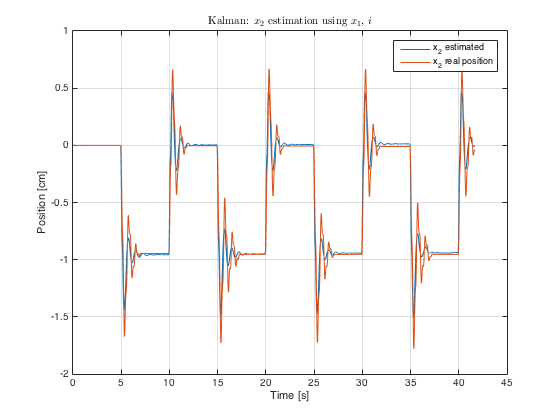
\includegraphics[width=\linewidth]{img/filtering_khlm_021m_x1i_to_x2.png}
\caption{Estimate of the second cart position using $i,x_1$. On the first cart there are 0 masses, on the second one there are two, and on the third one there is only one. The spring setup is $K_h, K_l, K_m$.}
\end{minipage}
\hspace{\fill}
\begin{minipage}[t]{0.45\textwidth}
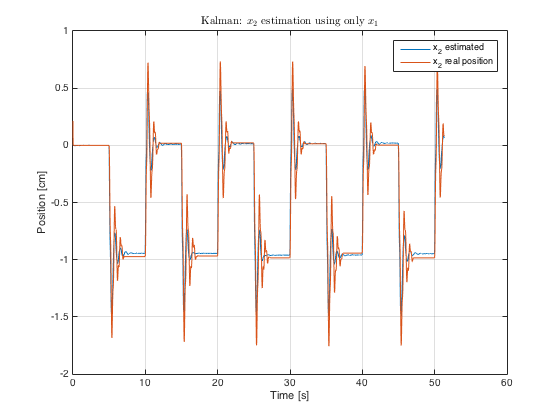
\includegraphics[width=\linewidth]{img/filtering_khlm_021m_x1_to_x2.png}
\caption{Estimate of the second cart position using $x_1$. On the first cart there are 0 masses, on the second one there are two, and on the third one there is only one. The spring setup is $K_h, K_l, K_m$.}
\end{minipage}
\label{fig:kalman_valid}
\end{figure}


\section{Extended Kalman Filter}
In this section we present the design of a filter which allows to estimate online the stiffness of a spring.\\

The setup is the one degree of freedom open loop model fed by a voltage, where the current and cart position can be sensed. The plant is described by the state-space model

\begin{equation}
	\dot{x}=\begin{bmatrix}
		-\frac{R}{L} &0 & 0 \\
		0 & 0 & 1 \\ 
		\frac{\gamma}{\hat{M}} & -\frac{K}{\hat{M}} & -\frac{C}{\hat{M}}
	\end{bmatrix}
	x
	+
	\begin{bmatrix}\frac{1}{L} \\ 0 \\ 0\end{bmatrix} v(t)
\end{equation}

and we suppose the value for $K$ is unknown and needs to be estimated online. We include $K$ as a state variable which is constant over time. The new system is nonlinear ($K$ multiplies $x_1$)

\begin{equation}
		\begin{bmatrix}
			\dot{i} \\
			\dot{x}_1 \\
			\ddot{x}_1 \\
			\dot{K} \\
		\end{bmatrix}
		= 
		\begin{bmatrix}
			-\frac{R}{L} i(t) \\
			\dot{x}_1 \\
			\frac{\gamma}{M} i - \frac{1}{M} Kx_1 - \frac{C}{M} \dot{x}_1 \\
			0
		\end{bmatrix}
		+
		\begin{bmatrix}\frac{1}{L} \\ 0 \\ 0 \\ 0 \end{bmatrix} v(t)
\end{equation}

and we want to observe the state so to obtain the value of spring stiffness $K$, making use of the extended Kalman filter (EKF). The filter has been designed in discrete time, hence the equations above has to be discretized wrt the sample time $T$.

\begin{eqnarray}
	\dot{x} \approx \frac{x(k+1)-x(k)}{T} = f(x) + Bv(k)
	\implies x(k+1) = x(k) + Tf(x) + TBv(k)
\end{eqnarray}

\emph{Matlab} does not provide an implementation for EKF and we needed to write it from scratch. We then designed a function which, given the current measurements of input $v(t)$ and output $i(t), x_1(t)$, outputs the state prediction $\hat{x}$. The \emph{Matlab} implementation is listed in the appendix.\\

The verification of the observer was performed on \emph{Simulink} making use of the scheme in figure which allow us to compare the true state with the observed one.\\

 
\begin{figure}[h]
\centering
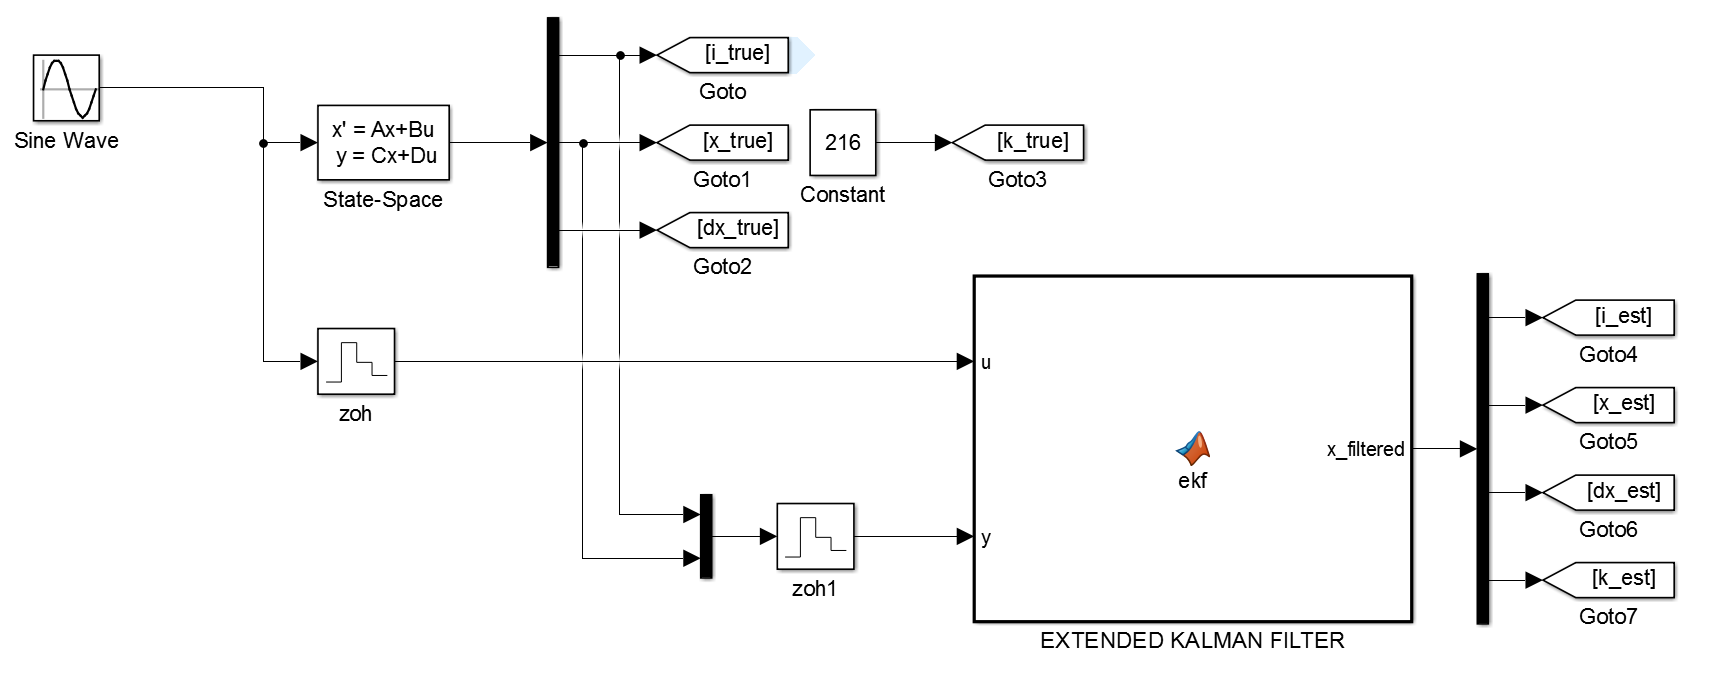
\includegraphics[width=0.7\linewidth]{img/ekf_scheme}
\caption{Simulink scheme used for verification.}
\label{fig:ekfscheme}
\end{figure}

The results are satisfactory as the unknown parameter is estimated with good accuracy.\\

\begin{figure}[h]
\centering
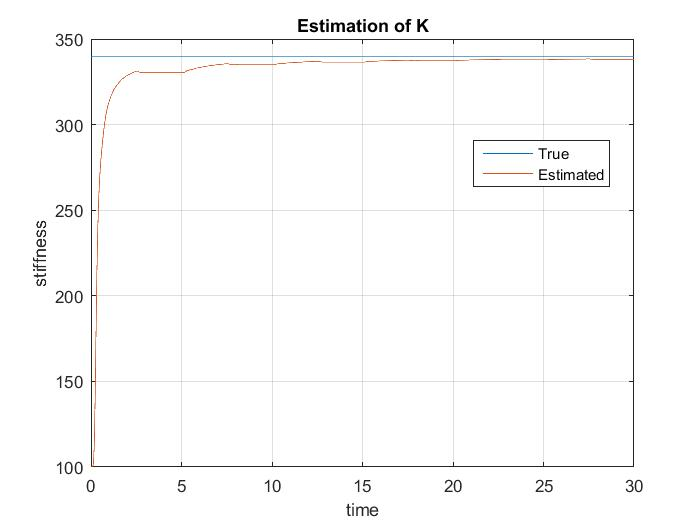
\includegraphics[width=0.7\linewidth]{img/ekf_sim}
\caption{$K$ estimation by feeding a train of pulses to the openloop plant.}
\label{fig:ekfsin}
\end{figure}

The system has then been ported onto Arduino and we ran the same experiment we performed offline. We expect the filter to converge to the same value as before but the transient might be different due to nonlinearities not included in simulink. The results are very satisfactory also in the online testing and resemble nicely the simulation.\\

\begin{figure}[h]
	\centering
	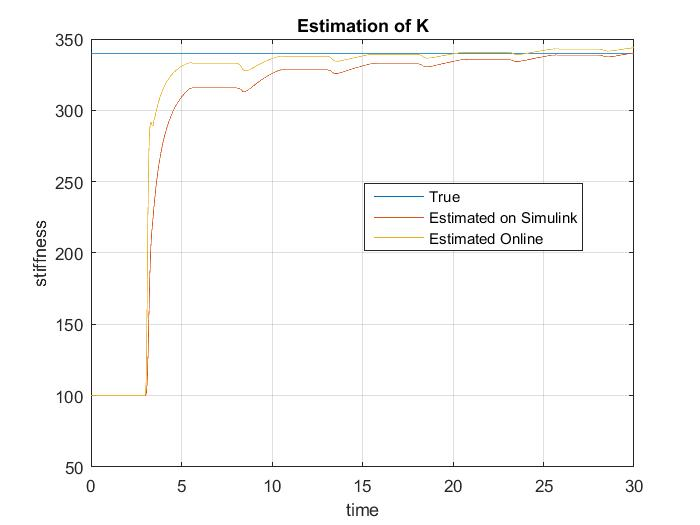
\includegraphics[width=0.7\linewidth]{img/ekf_ard}
	\caption{Online estimation by feeding a train of pulses to the openloop plant.}
	\label{fig:ekfard}
\end{figure}

The plot shown in figure \ref{fig:ekfard} has been obtained by measuring the output of the EKF on arduino and, as comparison, the output of the filter on \emph{Simulink} fed by the measured signal on the board in order to compare the outputs using the same data.
